\documentclass[letterpaper, 10pt, onecolumn, draftclsnofoot]{IEEEtran}

\usepackage[utf8]{inputenc}
\usepackage{listings}
\usepackage{geometry}
\usepackage{float}
\usepackage{enumerate}
\lstset{breaklines=true}
\geometry{margin=0.75in}
\usepackage{setspace}
\singlespacing
\usepackage{section}[placeins]
\usepackage{url}
\usepackage{array}
\usepackage{graphicx}
\usepackage{enumitem}
\usepackage{tabularx}
\usepackage{titlesec}
\titlelabel{\thetitle.\quad}
\usepackage{cite}
\usepackage{tabu}
\graphicspath{{./}}
\usepackage{booktabs}% http://ctan.org/pkg/booktabs
\newcommand{\tabitem}{\textbullet~~}

\usepackage[parfill]{parskip}



\renewcommand\thesection{\arabic{section}}
\renewcommand\thesubsection{\arabic{section}.\arabic{subsection}}
\renewcommand\thesubsubsection{\arabic{section}.\arabic{subsection}.\arabic{subsubsection}}

% THIS SHOULD BE A GOOD TEMPLATE FOR US TO FOLLOW.
% THE LAYOUT IS TAKEN FROM THE I.E.E.E. STD. 1016-2009 - ANNEX C 'TEMPLATE FOR AN SDD'.
% I KNOW IT'S WEIRD TO HAVE THE REFERENCES AND SUMMARY AT THE TOP, BUT THAT'S HOW THESE DOCS ARE I GUESS.
% -A

% TITLE / AUTHOR DATA
\title{\Large{\textbf{AR Sandbox for Construction Planning \\
                      Traffic Simulation Feature Update \\ 
                      \large{Design Document}}} \\
                      \vspace{5pt}
                      \small{Prepared for Dr. Joseph Louis \\
                      Oregon State University \\
                      School of Civil and Construction Engineering}\\
                      \today}
                      
\author{Team Augmented Construction Education \\
       McKenzie~Gray,~Jonah~Spencer,~Adam~Sunderman}

% DOCUMENT BEGIN
\begin{document}

% SECTION TITLE
\maketitle
\vspace{30pt}
\begin{center}
\begin{tabular}{@{}p{.5in}p{4in}@{}}
Approved: & \hrulefill \\
& \hspace{10em} \\
Date: & \hrulefill \\
& \hspace{10em} \\
& Joseph Louis, Ph.D.\\
& Assistant Professor of Civil and Construction Engineering \\
& Oregon State University \\
\end{tabular}
\end{center}
\vspace{50pt}

% SECTION ABSTRACT
\begin{abstract}
    This paper describes proposed changes to a currently operating Augmented Reality (AR) Sandbox located at Oregon State University. AR sandboxes have been developed all over the country for both educational and entertainment purposes and the basic concept behind the sandbox is simple. The unit is comprised of a physical box of sand, a video projector, a depth sensor, and a computer. As users interact with the AR Sandbox and shape the sand within, they will also manipulate in various ways images projected onto the sand. Most often, these images are topographic and elevation maps displayed over the sand. The changes described in this document will add new functionality to the AR Sandbox in the form of a new marker-based system which allows users to add three-dimensional elements to digital scenes projected within the AR Sandbox. These scenes will be used to run traffic simulation on sections of roadway that model an area currently under construction. The main goal of this project is to create an interactive tool for civil engineers to learn about and explore transportation engineering.  
\end{abstract}
\newpage
\tableofcontents
\clearpage
\newpage

% SECTION CHANGELOG
\section{\textbf{Change Log}}
\renewcommand{\arraystretch}{4}
\begin{center}
    \begin{tabular}{|p{4cm}|p{6cm}|p{6cm}|}
        \hline
        \textbf{\large Section} & \textbf{\large Original} & \textbf{\large New} \tabularnewline
        \hline
        \textbf{Scope} & 
        \tabitem Original scope too broad, very unspecific. & 
        \tabitem Updated scope to include specific features and components. \tabularnewline
        \hline
        \textbf{Glossary} & 
        \tabitem The definition for markers specified the use of markers for placing objects in the scene. \newline
        \tabitem The definition for virtual buttons was incorrect. &
        \tabitem Changed the definition of markers to be more generic.  \newline
        \tabitem Corrected the definition for virtual buttons. \tabularnewline
        \hline
        \textbf{Data Design} & 
        \tabitem Road networks data defined incorrectly. &  
        \tabitem Updated to reflect better understanding of SUMO's network tools. \tabularnewline
        \hline
        \textbf{Component Diagram} & 
        \tabitem Road network data explained incorrectly. \newline
        \tabitem Road network creation explained incorrectly. \newline
        \tabitem Included subsection for Scene Creation Mode. & 
        \tabitem Updated description. \newline
        \tabitem Updated description. \newline
        \tabitem Removed subsection for Scene Creation Mode. \tabularnewline
        \hline
        \textbf{Virtual Buttons} & 
        \tabitem The description of the operation of virtual buttons was incorrect. \newline
        \tabitem Included a bullet point for "loading new markers and models into the system" with virtual buttons. & 
        \tabitem Corrected the description of the operation of virtual buttons.  \newline
        \tabitem Removed the bullet point for "loading new markers and models into the system" with virtual buttons. \tabularnewline
        \hline
    \end{tabular}
\end{center}
\newpage

% SECTION INTRODUCTION
\section{Introduction}
    \subsection{Purpose}
        The purpose of the AR Sandbox is mainly educational and meant as a means to visualize large-scale construction projects. The AR Sandbox offers a new and unique way for students to visualize the topics about which they learn in class with real-time feedback supported by various augmented reality modules.
        
    \subsection{Scope}
        The system currently contains several modules for performing various tasks within the AR Sandbox. These modules include a cut-and-fill mode for calculating earth moving requirements for large transportation projects, a topographical mode for displaying current sand height information within the sandbox, and a design mode for projecting and editing sections of roadway.\\
        The proposed upgrade will add modules giving users the ability to create full road networks and run traffic simulations in the AR Sandbox. The traffic simulations and old modes of operation will be built and re-designed respectively for user interactions with Vuforia Augmented Reality. Markers, which are distinguishable by Vuforia, will be used to indicate the type of operation the user want to perform.
        
    \subsection{Context}
    \begin{center}
        See Appendix \ref{ARSandboxDiagram}
    \end{center}
% SECTION GLOSSARY
\section{Glossary} 
    \begin{enumerate}[label=]
         \item {\textbf{Augmented Reality (AR):} A way of mixing computer images with the user’s vision. AR refers to the graphics displayed over the sand. When a user manipulates the sand, the graphics displayed on the sand will change.} 
         
        \item {\textbf{AR Sandbox:} Augmented reality sandbox. A physical sandbox with a depth sensor and projector that displays graphics on the sand, such as roadways and ground topography.}
        
        \item {\textbf{CPU:} Central Processing Unit. The computer component that handles general processing instructions.}
         
        \item {\textbf{Depth Sensor:} A digital imaging device which uses a grayscale image to represent the distance from the sensor to the nearest surface.}
        
        \item{\textbf{Game Engine:} A program or set of programs designed to enable game developers to create games. A game engine helps manage and facilitate various game features and tasks such as graphics rendering, input devices, audio, physics, scripting and networking.}
        
        \item {\textbf{GPU:} Graphics processing unit. A computer component that handles graphics processing.}
        
        \item \textbf{Heightmap:} An image in which each pixel stores its displacement, or "height," from the ground.
        
        \item {\textbf{Markers:} Markers are physical objects that a user can place and move within in the AR Sandbox. Image recognition will allow markers to interact with the system in various ways.}   
        
        \item \textbf{Mass-Haul Diagram:} A diagram used to determine the most efficient way of moving earth in order to create the desired topology. 
        
        \item \textbf{Mass-Haul Simulation:} Excavation simulation; amounts of earth (dirt, rock, etc.) that must be moved, removed or brought into a location in order to create an acceptable terrain for a project.
        
        \item {\textbf{Projection:} The image cast on the sand's surface by the projector.}
        
        \item \textbf{Road Network:} A connected mesh of roads and traffic control devices.  
        
        \item {\textbf{SDK:} Software Development Kit. A set of software development tools used to create software for a particular platform or framework. For example, an AR SDK would provide tools necessary to create AR applications.}
        
        \item{\textbf{Shader:} A specialty program for graphics that tells the computer how to render (display) each pixel in an image.}
        
        \item \textbf{Simulators:} Software that use mathematical models to provide a realistic imitation of real-world behaviors.
        
        \item \textbf{Traffic Simulation:} A program inside a simulator that imitates traffic behaviors and patterns of users.
        
        \item \textbf{Microscopic Simulations:} Traffic simulations based on driver-centric simulation models that have individual agents (drivers) making decisions based only on information a particular agent has.
        
         \item \textbf{Macroscopic Simulations:} Traffic simulations based on mathematical models that are derived from multiple microscopic simulations and real-world flow pattern data.
    
        \item \textbf{Mesoscopic Simulations:} Despite being based on simulating individual cars, each car's behaviour is based on a car-following model, which can be solved efficiently using an event-based approach. They perform more efficient simulations than microscopic simulations while not having the overhead of microscopic simulations.
        
        \item \textbf{Terrain Mesh:} A three-dimensional object created based on the heightmap produced by the depth sensor. This object can be used in scenes in Unity game engine to interact with other objects. This will create the ground on which a scene is built. 
        
        \item {\textbf{Topography:} The surface elevation features of the sand in the AR Sandbox at any given time. Measured from all points in the AR Sandbox and projected as a color gradient from red to blue that covers the sand's surface.}
        
        \item \textbf{Traffic Control Devices:} Devices used to control traffic patterns of vehicles and pedestrians alike. Examples include: Stop Lights, Yield Signs, Crosswalks, and Construction Zones, among others.
        
        \item {\textbf{Virtual Buttons:} Virtual buttons are digital objects that can be attached to markers. They are interacted with by touching the corresponding location on the marker.} 
        
        \item \textbf{Virtual Camera:} A component of a virtual scene that determines from which perspective the scene is viewed.
        
    \end{enumerate}

% SECTION DATA DESIGN
\section{Data Design}
    \subsection{Heightmap}
        The AR Sandbox uses data received from the depth sensor to create a topographical projection on the surface of the sand in real-time. A heightmap is a way to save this depth data as a grayscale image. Each pixel in the image has a value from 0 to 255 which determines the shade of the pixel in the image. This shade directly correlates to the height of the terrain from which the data was read. As such, heightmaps will be utilized to represent and store data related to topographical information in the AR Sandbox.  
    \subsection{Terrain Mesh}
        A terrain mesh will be generated by the Unity game engine from the heightmap. This mesh is a three-dimensional object which represents the surface of the sand in the AR Sandbox. This is the object that will be visible to the end user and projected onto the sands surface.  
    \subsection{Scenes}
       Scenes will be created in the Unity game engine in a similar way to levels in a video game. Once the terrain's height information has been processed, a new scene will be created which will be used for scene building and traffic simulations. Scenes will be a composition of all pieces of data the AR Sandbox has available. A scene will have a starting heightmap that is always saved with the scene as well as a current heightmap that saves any user-made changes. The terrain mesh generated from this heightmap will be used for placement and orientation three-dimensional models to be added to the scene by the user.
     \subsection{Three-Dimensional Models}
        The AR Sandbox will have a collection of pre-built, three-dimensional models that will be called upon during scene creation. These models will be purchased from the Unity Asset Store. Special models may need to be created with Blender if there is a need that cannot be filled by the Asset Store.
    \subsection{Road Network}
        New road networks will be generated with SUMO then converted into a 3D models for display in Unity. Each road network will have a scene associated with it. 
    
% SECTION COMPONENT DESIGN
\section{Component Design}
    \subsection{System Structure}
        \begin{center}
            See Appendix \ref{ComponentBlockDiagram}
        \end{center}

    \subsection{Component Diagram}
        \begin{center}
            See Appendix \ref{ComponentFlowDiagram}
        \end{center}
        
        \subsubsection{Depth Sensor API}
            Microsoft's Kinect depth sensor API will handle reading current terrain heights in the AR Sandbox. Then, the height data will be  translated to a heightmap that can be used to render the terrain and scene.
       
        \subsubsection{Geometry Interpreter}
            The geometry interpreter handles translating a heightmap into a three-dimensional mesh that can be used in the Unity game engine to create and render scenes.  
        
        \subsubsection{Height Look-up}
            The height look-up component will handle requests for height data from a heightmap. A heightmap stores three-dimensional data in a two-dimensional format. Height look-up converts this two-dimensional data to a three-dimensional data format that can be used in Unity and other three-dimensional software.
       
        \subsubsection{Object Recognition API}
            Object recognition will be achieved using the Vuforia SDK. Images to be recognized will be saved in Vuforia's Target Manager. Any images in the Target Manager can then be used to create markers that are recognizable to Vuforia. Once an image is saved in the Target Manager, an Image Target can be created within the Unity Editor. Image Targets can be connected to game objects whose locations are based on the locations of the corresponding Image Targets and which can otherwise be used like any other game object.
       
        \subsubsection{Vertex/Fragment Shaders}
            The vertex and fragment shaders are responsible for applying colored elevation data onto a terrain mesh. Shaders use height data from the heightmap to determine the color of the mesh at each point. Depending on the current mode of operation, standard elevation heights or differences in height may be rendered. When loading a saved terrain, the shaders will depict the difference between the sand in the AR Sandbox and the height data from the saved terrain. In normal operation the shaders will just display the difference between various points in the AR Sandbox.
       
        \subsubsection{Traffic Simulation Mode}
            The traffic simulation mode will load and run a created road network. The objects that describe a scene such as roads, vehicles, and buildings will be built as 3D objects and placed on a terrain sized appropriately for the network. As the simulation runs various functions will be available for the user call using Vuforia markers. For instance a user will be able to add and remove work zones on roads, interact with traffic lights, and change simulation parameters such as displaying Mesoscopic and Microscopic simulations (see glossary).  
        
        \subsubsection{Traffic Simulator}
            Traffic simulation will be achieved using the Simulation of Urban Mobility software suite (SUMO) running as a background process. Road networks will be fed into SUMO after they have been generated. When a simulation mode has been selected, the simulation will send output display data to an XML file. The Unity application will then read that XML data and update car positions accordingly.
       
        \subsubsection{Traffic Simulation API}
            To interact with, and get data from, the traffic simulator (SUMO) we will create a traffic simulator controller class as an API. This controller will be able to: generate road networks, load road networks, edit existing road networks, specify simulation modes, and read simulation output. The API will allow us to separate our concerns when talking to the SUMO and reading simulated data.
       
        \subsubsection{Road Network Importer}
            SUMO's NETCONVERT takes in premade networks from other applications, and converts them to SUMO-style networks\cite{SUMO}. In addition, SUMO may use a heightmap to convert a two-dimensional network into a three-dimensional network. 
       
        \subsubsection{Marker-Based Road Network Editor}
            To edit an existing road network, the Marker-Based Road Network Editor will use Object Recognition to determine predefined markers and their locations. When the location is determined, the system will match that object to the node in the Road Network on which it is placed and perform a predefined action related to that object. I.E. if the object is defined to be a construction zone of a given length, the system will alter that section of road to be a construction node, and reload the network to SUMO to relaunch the simulation. 
        
        \subsubsection{Mass-Haul Mode}
            Mass-Haul mode will create a Mass-Haul Diagram and a difference map based on the topography of the sandbox and the desired topography. This diagram will show red where sand needs to be removed and blue where sand needs to be added. This difference can be used with the generated Mass-Haul Diagram to demonstrate how to follow a Mass-Haul Diagram. 
        
        \subsubsection{UI}
            The UI for the AR Sandbox will consist predominantly of markers used to interact with the AR scene. The design details for the UI are described in the following section.
        
        \subsubsection{Renderer}
            Scenes will be rendered by the Unity engine. Objects making up the scene will be viewed by a virtual camera within Unity, and this view will be projected into the sandbox. Any changes made to the scene will be routed through the scene in Unity and rendered accordingly.
            
% SECTION UI DESIGN
\section{User Interface Design}
    \subsection{Markers}
        Users will interact with the AR Sandbox primarily using physical markers. Markers will consist of flat objects with two-dimensional images representing different objects in the scene. Specifically, one marker will represent traffic lights, one marker will represent a stop sign, and one marker will represent a construction zone. Users will be able to place these markers into the sandbox in order to add the corresponding arbitrary object to the scene.
        
    \subsection{Virtual Buttons}
        Menu navigation will be accomplished using virtual buttons. Like markers, virtual buttons allow for physical interaction with digital objects. Virtual buttons are attached to markers and can be interacted with by touching the correct part of the image that makes up the marker. With virtual buttons, users will be able to navigate menus in a familiar way, but without needing to use a mouse. This menu navigation will be necessary for:
        \begin{itemize}
            \item Selecting system modes
            \item Changing mode-specific settings
            \item Calibrating the display area
            \item Simulation interactions
            \item Saving and loading scenes
        \end{itemize}

%SECTION APPENDICES
\newpage
\appendices
    \section{AR Sandbox Diagram}
    \label{ARSandboxDiagram}
        \begin{center}
        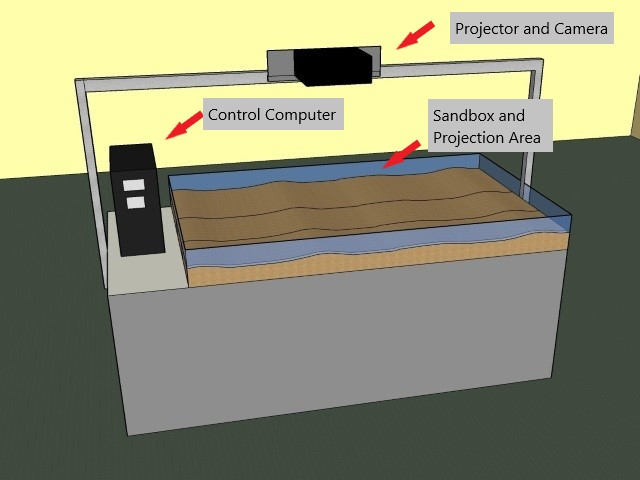
\includegraphics{ARSandbox.jpg}
        \end{center}
    \section{Component Block Diagram}
    \label{ComponentBlockDiagram}
        \begin{center}
        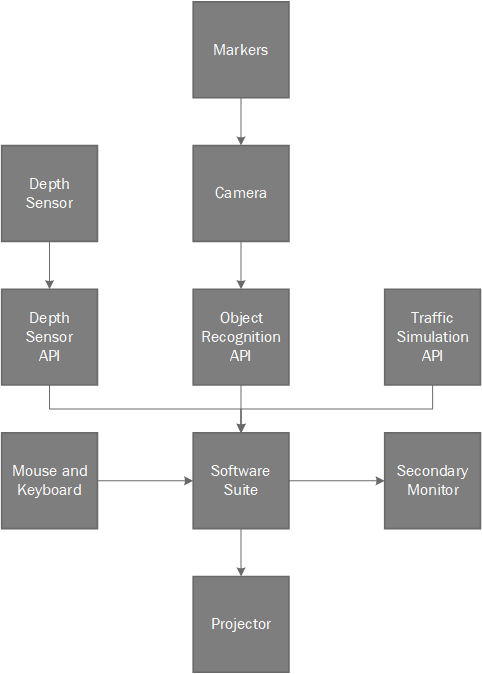
\includegraphics{BlockDiagram.png}
        \end{center}
    \section{Component Flow Diagram}
    \label{ComponentFlowDiagram}
        \begin{center}
        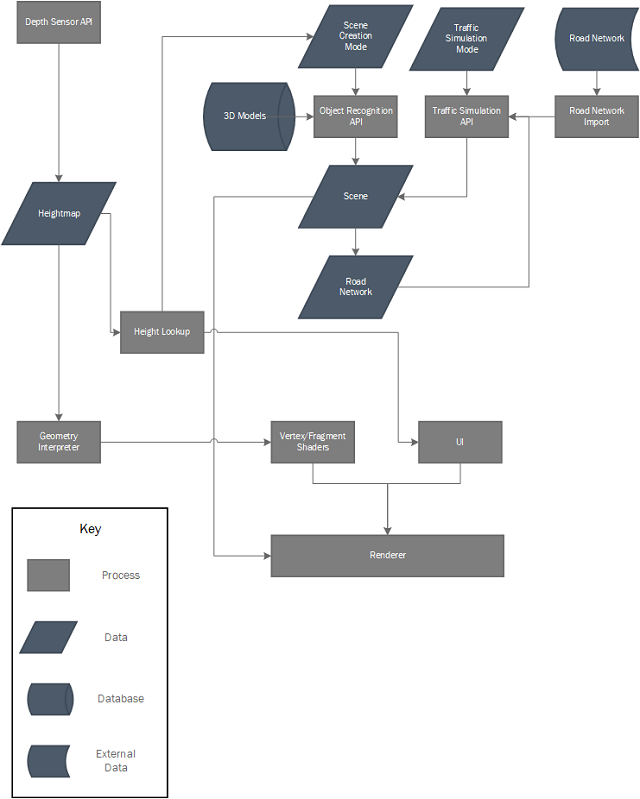
\includegraphics{ComponentFlowDiagram.png}
        \end{center}

%SECTION REFS
\newpage
\nocite{*}
\bibliographystyle{IEEEtran}
\bibliography{references}
        
\end{document}
